\documentclass{ltjsbook}
\usepackage{docmute} 
\usepackage{../myStyle} 

\begin{document} 
\chapter{記述統計量} 
\label{chapter4} 
\section{はじめに}
さて，ここまでで心理学においてなぜ統計学が必要か，計算機とはどういうものか，計算機に与えるデータはどういうものか，という話をしてきました。下準備はそこまでです。いよいよ，今回から心理統計の具体的な話に入っていきます。

初めに，心理統計の3つの枠組みを紹介しておきます。
\begin{description}
    \item[記述統計 descriptive statistics] データの特徴を記述する統計法。可視化，代表値による要約など。 データを取ったらまずやるべき作業がこちら。手元のデータでわかることを，隅々まで書き表すのが狙いです。
    \item[推測統計 inferential statistics] 部分的なデータから全体像を推測する統計学。心理統計の目的は一部のサンプルから全体を予測することにあるのです。この授業の後半(後期)は主にこの話になります。
    \item[多変量解析 multivariate analysis] 大量のデータから意味のある情報を引き出す，あるいは無意味な情報を削ぎ落とす技術です。調査研究をする場合はもちろん，センサーなどの機器から大量に取れるデータを扱う場合にも使われる技術です。データサイエンス，機械学習(いわゆるAI)などにも通じる領域です。本学では2年のデータ解析応用で扱います。
\end{description}

ということで，ここにあるように記述統計学が最初のステップになります。手元にあるデータの特徴を記述することが目的になります。記述という意味では可視化もそうなのですが，今回は数字によってデータの特徴を記述することを考えます。複数のデータの代表的な値ですから，代表値と言われたりします。

研究対象を数値化したとしましょう。それを眺めて「いろいろな数字があるなあ」と感心していたのでは，数値化した意味がありません。得られた\textbf{データは図にする}のが基本です。すぐに図にします。いろいろな図にします。前回も話しましたが，とにかく図にします。しなければなりません。さて，図を見て考えをまとめるのが重要なのですが，具体的にどういう特徴があるのか，あるいはどういう違いがあるのかといったことを，要約して表現できればなお良いですね。そこで代表値を考えることになります。

いきなり身も蓋もないことをいうようですが，たくさんの数値を1つの代表値を使って記述する，というのは基本的に無理があります。十人十色，いろいろな違いがあるからこそ，そのデータセットは意味があるのに，たった1つの数字に変えて表現するのですから。代表値は，何らかの側面で評価することで一つに定まるものであって，あくまでもその評価次元での代表値に過ぎません。つまり，一つの代表値だけで全体が分かるわけではないのです。あるいは，一つの代表値にするということは，少し無理をして情報を削ぎ落とすということでもあります。代表値は何であれ，必ず何らかの情報が欠け落ちているのです。ですから，統計データを扱うときは，複数の代表値を使って多角的に判断するのが基本です。そのことをまずしっかり理解しておいてください。

その上で，代表値を2つの種類に分けて説明します。ひとつは中心化傾向の指標，もうひとつは散らばりの指標です。

\section{中心化傾向の指標}
\subsection{平均値mean}

\textbf{平均値mean}\footnote{英語ではaverageというのも平均を意味します。meanの方がより意味が狭く，averageはより広い意味で代表的であるという違いがあるようです。}，より正確には算術平均\footnote{他にも調和平均，幾何平均などがあります。}は最もよく知られた代表値でしょう。計算方法は，全てのデータをたしあわせて，足したデータの個数で割る，というものです。

図\ref{fig::04_01}に5人の所持金を示しています。この例では，平均値は次のように計算できますね。
$$ (15000+30000+20000+10000+20000)/5=19000$$

\begin{figure}[ht]
    \centering
    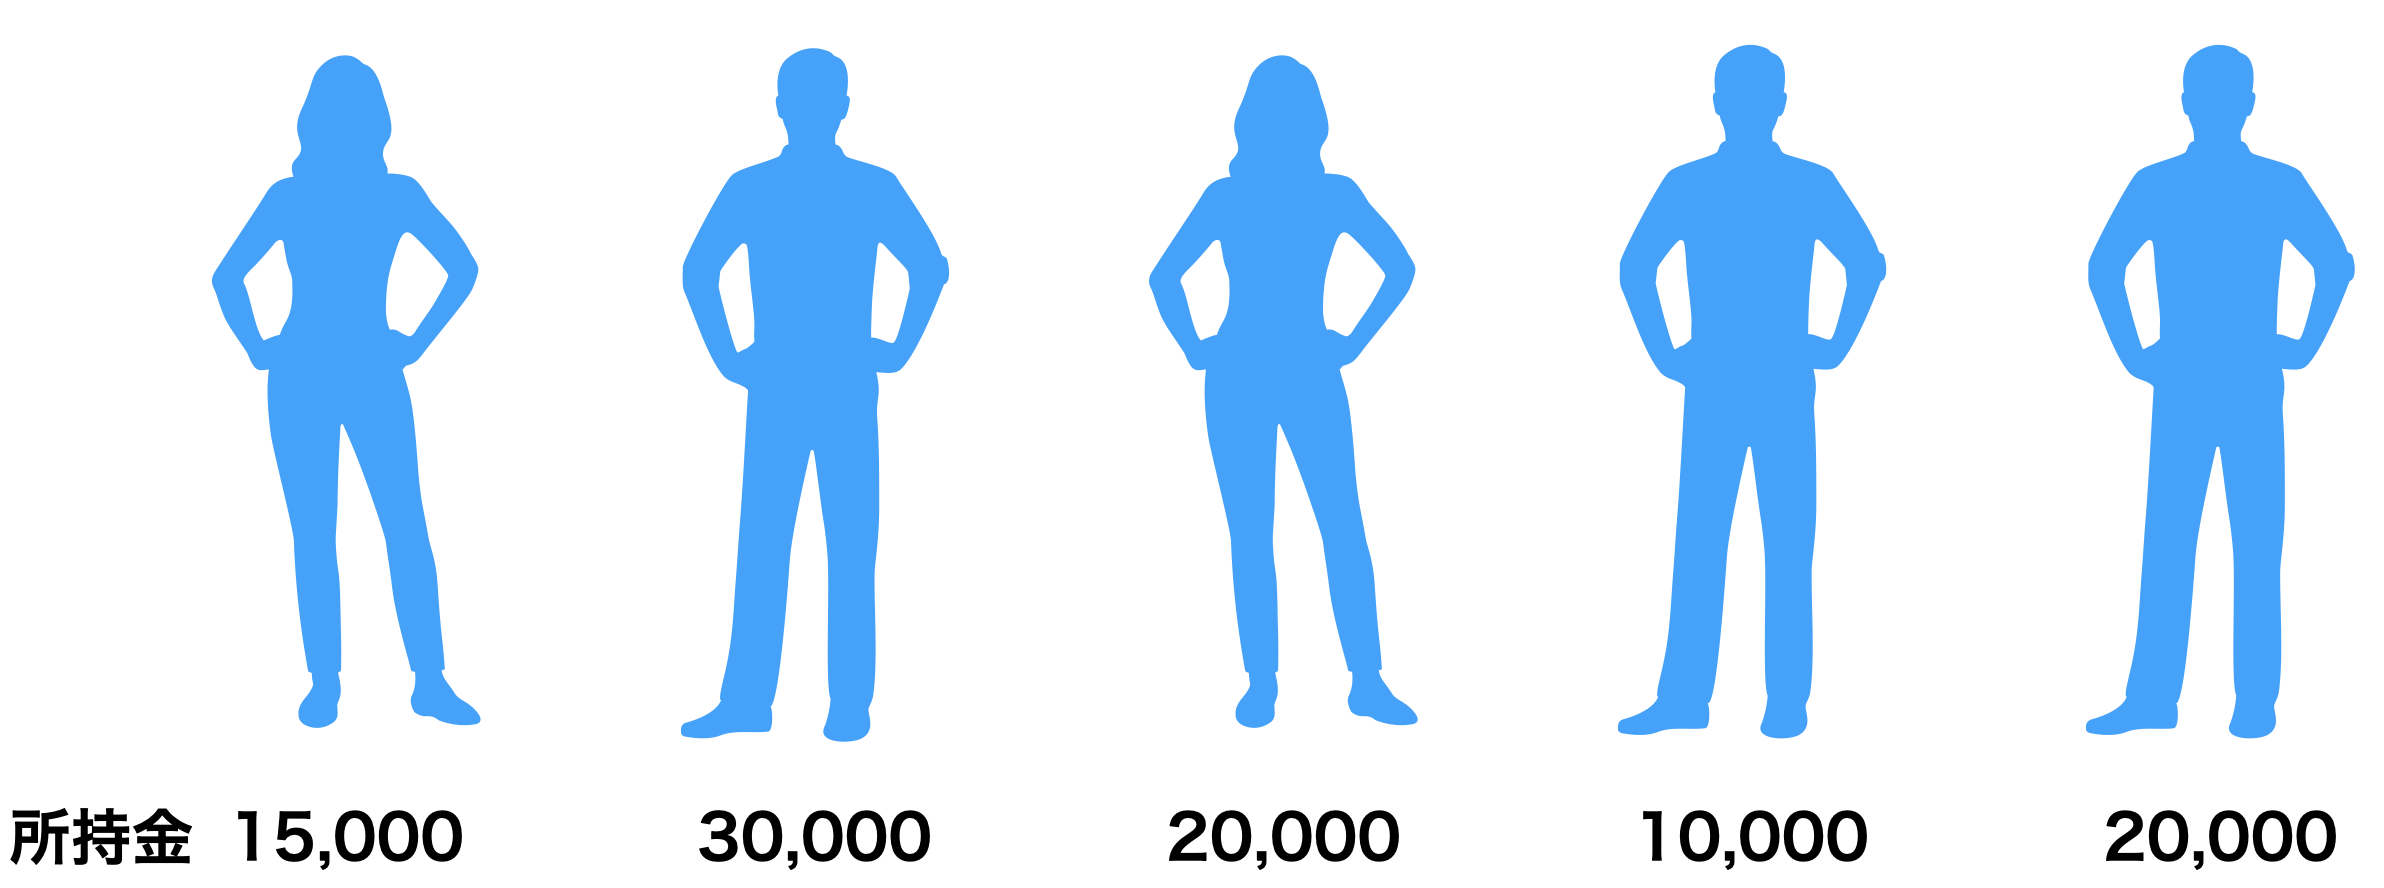
\includegraphics[keepaspectratio,width=12cm]{images/text04/slide04_01.png}
    \caption{5人の所持金データ}
    \label{fig::04_01}
\end{figure}

\paragraph{文字と記号の導入}
さてこれを，今後のために記号で一般的に表記する方法について知っておきましょう。
変数は一般に$x$や$y$で表されます。
今回は5人分のデータがありますが，1人目のデータ，2人目のデータ，といった違いを表すときは$x_1,x_2,\cdots$のようにアルファベットの右斜め下に小さく数字を添えます。添字と言います。
さて今回は所持金という1つの変数でしたが，2つ目の変数，三つ目の変数・・・とたくさんのデータが手に入ることもあります。そのようなとき，変数は$x_{ij}$と添字を2つ書いて表現します。ここで$i$がケース(個体，観測番号)を表し，$j$が何番目の変数であるかを表す，というルールにします\footnote{この講義ではこのルールで通します。必ずしも個体が前で変数が後，という決まりがあるわけではありませんが，このような記号を導入するときはどの文字が何に対応しているか明記することが一般的です。この講義で特に明記していなければ，前の添字が個体で後ろの添字が変数を表すのだと思ってください。}。

次に足し算の記号を紹介します。$\sum$で総和を表すことにします。この記号はギリシア文字の大文字のSで，足し合わせるsummationの頭文字をとって$\sum$，サムと読みます。この記号には上と下に文字を追加して，次のような意味で使います。
$$\sum_{i=1}^5 x_i= x_1 + x_2 + x_3 + x_4 + x_5 $$
ここにあるように，$\sum$の下に$i$という文字があります。この文字$i$が$1$から始まって$5$まで変化し総和する，という薄学記号です。$\sum_{i=1}^5 x_i$の$x_i$という変数について，$i$が1から5まで変わるわけですから，右辺にあるように添字が変わりながら全て足し合わせる，という意味の記号です。この$\sum$も，文脈から考えてどこからどこまで足すのかが明らかな場合，上下の添字は省略されることがあります。

さて，先ほどの5人の平均ですが，足し算の場所は$x_1+x_2+\cdots+x_5=\sum_{i=1}^5 x_i$と書けます。これを5で割れば平均になりますから，$\frac{1}{5}\sum x_i = 19000$というわけです。このように記号で表現しておくと，平均値は一般に次のように表すことができます。

$$ \bar{x} = \frac{1}{N}\sum_{i=1}^N x_i $$

今回は5人でしたが，一般に$N$個のデータを扱うときにまで拡張できました。左辺は平均値$\bar{x}$で，エックスバーで表すことが一般的です。
\subsection{中央値median}
次の代表値は\textbf{中央値median}です。データを大きさの順に並べて行って，ちょうど真ん中のケースの値をその代表値として使う，というものです。先程の図\ref{fig::04_01}の場合は，並べ替えると$10000<15000<20000=20000<30000$となります。上から3番目(下からでもいいです)が20000円ですから，中央値は20000円ということになります。

今回はたまたま，5人のケースですから真ん中は3番目となりましたが，データの数が偶数しかなかったらどうするか，という問題があります。その場合は，真ん中に来た2つの値の算術平均でもって中央値とすることが一般的です。

\subsection{最頻値mode}
最後に\textbf{最頻値mode}についてです。漢字の成り立ちからわかるように，頻度が最も多いものを代表地とするのが最頻値です。先程の図\ref{fig::04_01}の場合は，10000円が1人，15000円が1人，30000円が1人ですが20000円持っている人が2人いましたので，最頻値は20000円になります。

このように，データの中心をどのように考えるかによっても3つも考え方があり，それぞれが一致するわけではないのです。それぞれの意義がありますので，見比べながら考える必要があります。

では練習です。次の表\ref{tbl::04_01}のようなデータがあった場合，平均値，中央値，最頻値はそれぞれどうなるでしょう？

\begin{table}[ht]
    \centering
    \caption{5人の所持金データその2}
    \begin{tabular}{lllll}
        A& B & C & D & E\\\hline
    10000 & 10000 & 20000 & 25000 & 100000 \\
    \end{tabular}
    \label{tbl::04_01}
    \end{table}

この場合，平均は33000円，中央値は20000円，最頻値は10000円となりました。平均値が他の2つより大きくなりましたね。これは\textbf{外れ値outlier}があるからです。Eさんが，平均値をぐっと押し上げているのです。平均値は量的な中心をとりますので，1人でも遠く離れたところに位置すると全体的に中心が引っ張られます。中央値は順番の情報しか使いませんので，大金持ちが1人いても1位だ，と判断するだけです。最頻値は度数の問題ですので，大金持ちが1人いても度数1にしかなりません。平均値は外れ値に弱い，あるいは中央値や最頻値がそれに強いというだけです。

では平均値は使い物にならないのでしょうか？もちろんそうではなくて，左右対称に散らばっているようなデータであれば，平均値は良い代表値になります。データの散らばりが左右対称ではなく歪んでいるようであれば，平均値は適切な代表値になりません。

図\ref{fig::04_02}は，厚生労働省による「国民生活基礎調査」で示されたデータです\footnote{https://www.mhlw.go.jp/toukei/saikin/hw/k-tyosa/k-tyosa19/dl/03.pdf}。これを見ると所得分布は左側に歪んでおり，平均値は552万3千円ですが，中央値は437万円，最頻値は200-300万円のクラスということになります。最頻値は一番データ点が多いところですので，「国民の平均所得は552万円です」と言われると多くの人が(この例では少なくとも55.9\%の人が)，「えっ，私の年収低すぎ・・・?」という印象を抱きます。もちろん所得分布が低い方に歪んでいる状況も悪いのですが，代表値として平均値を使うことがそもそも適切でない例ともいえます\footnote{もちろん為政者の目から見れば，平均は550万円もあるんだから日本は豊かだ，とアピールできるので良い指標なのかもしれません。数字に悪意はなく，何の数字をどのように使うのかという人の側に問題があるだけです。}。ニュース報道などでは平均値しか報道されませんが，それでは不当な印象を与えることになります。\textbf{データは図にする}ことが大事なのです。
\begin{figure}[ht]
    \centering
    
\includegraphics[keepaspectratio,width=12cm]{images/text04/slide04_02.png}
    \caption{所得金額階級別世帯数の相対度数分布}
    \label{fig::04_02}
\end{figure}

ところで，最頻値は頻度を数えるものですから，間隔尺度水準以上の連続的な数字の場合はいくつかの区間に区切って数えることになります。図\ref{fig::04_02}の例もそうですね。ただしこの時，最頻値は区間幅の区切り方が違うと結果が変わってしまうことに注意しましょう。図\ref{fig::04_03}の2つのヒストグラムは，実は同じデータなのです。違いは区間幅binwidthのとり方で，左図は15点間隔，右図は5点間隔でグラフを書きました。最頻値はそれぞれ赤で囲ったところになりますが，左図の場合の最頻値は40-55点クラス，右図の場合は47-52点のクラスになります。最頻値の場合は，どのような区間幅でカウントするかということにも注意が必要ですね。
\begin{figure}[ht]
    \centering
    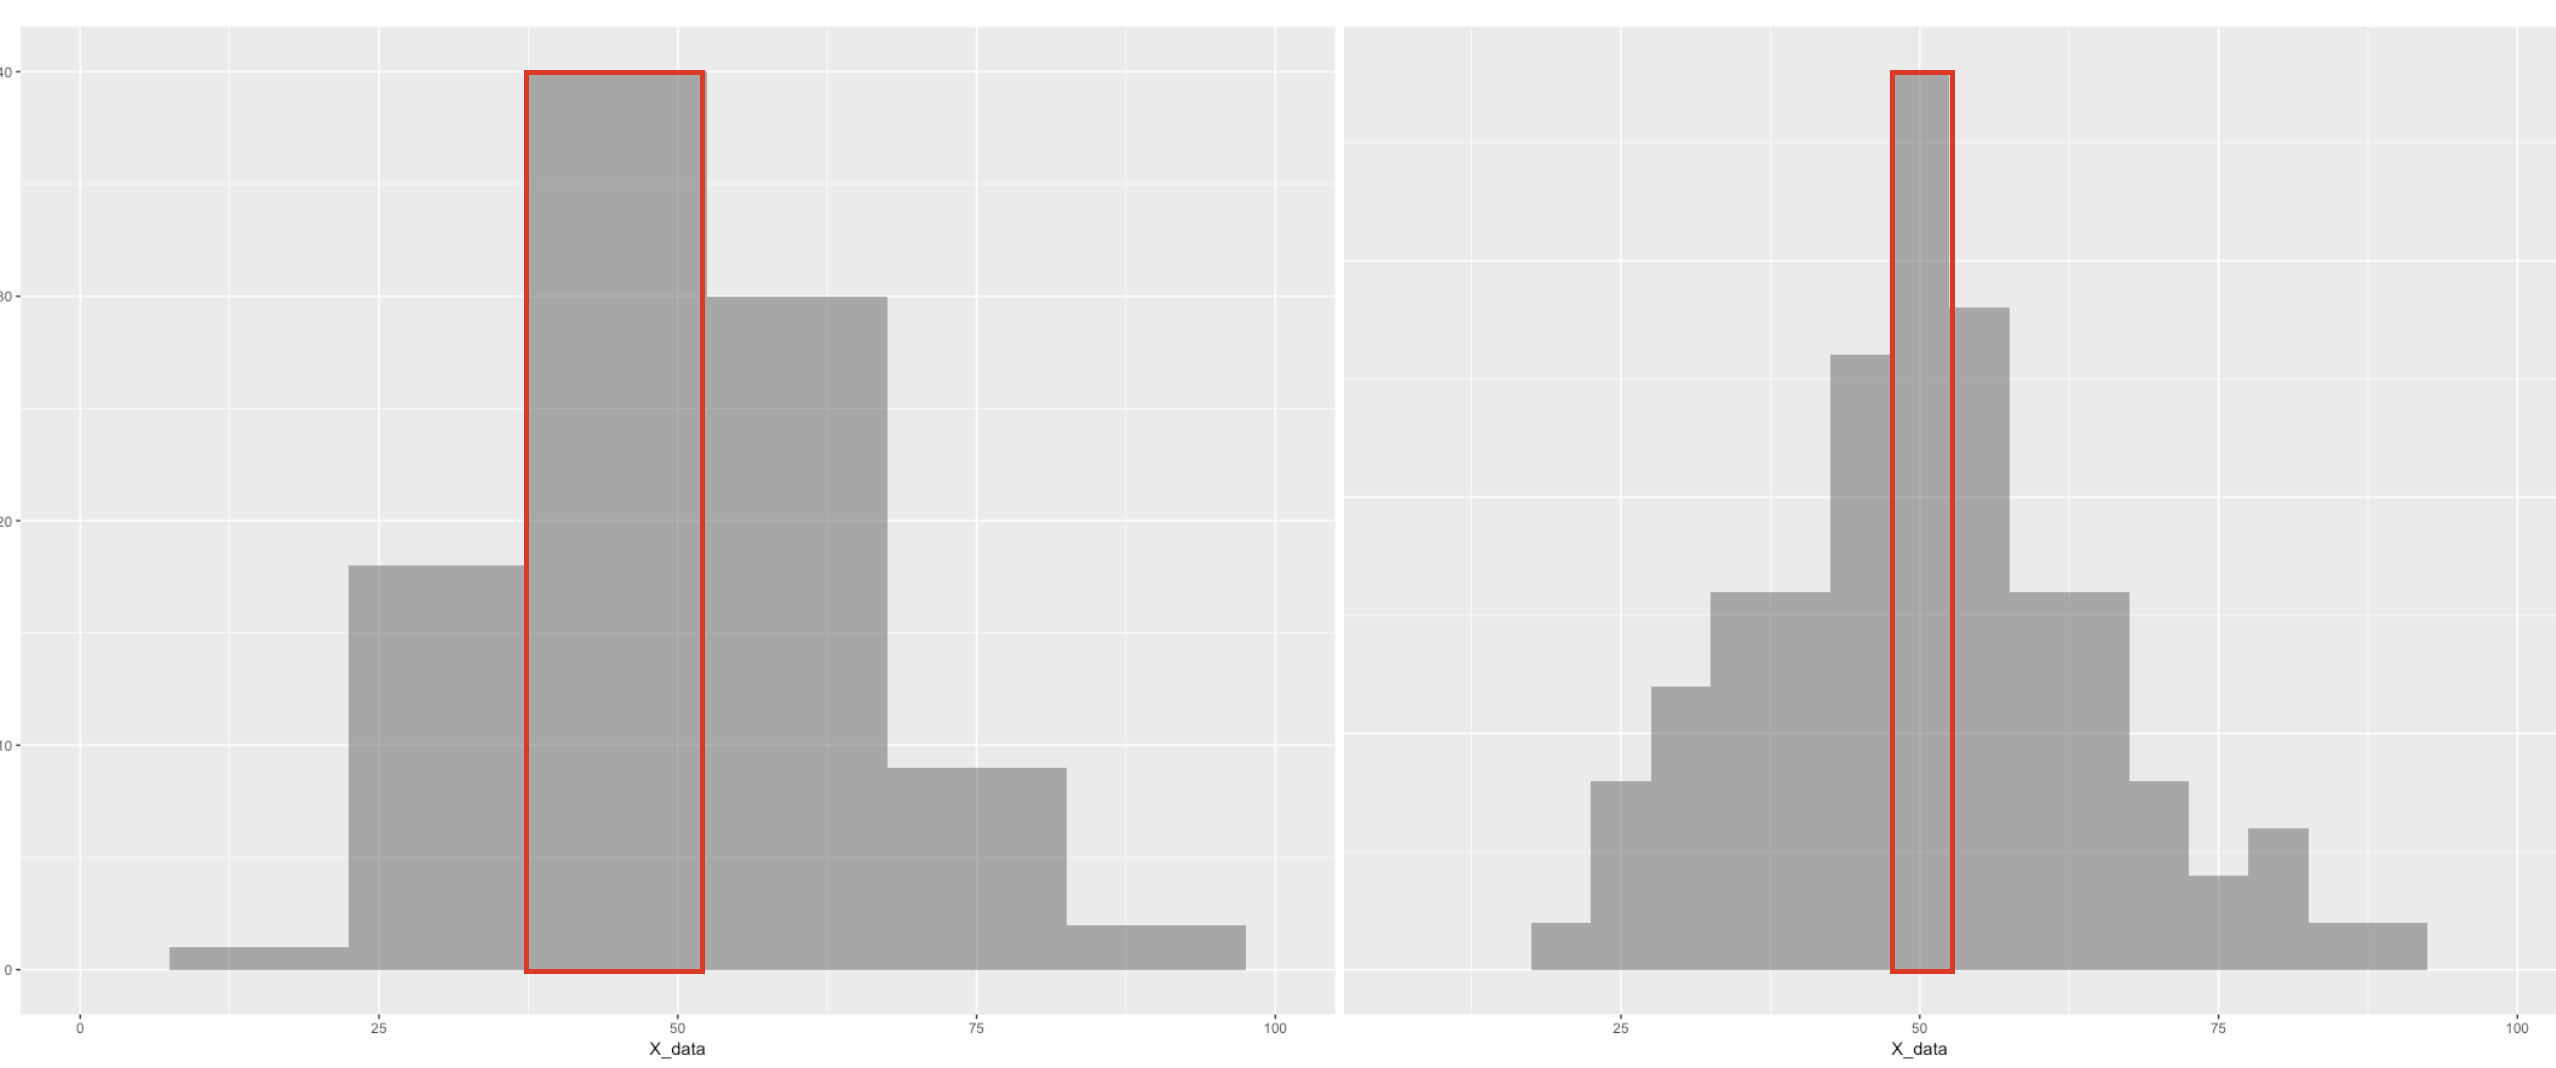
\includegraphics[keepaspectratio,width=12cm]{images/text04/slide04_03.png}
    \caption{区間幅の区切り方で結果が変わる}
    \label{fig::04_03}
\end{figure}

では，ここで出てきた3つの中心化傾向の指標を一旦まとめておきましょう。

\begin{description}
    \item[平均値] データを全部使って計算しており，外れ値がなければ全データが反映される良い指標。実際，統計分析で最も活躍している指標です。左右対称の分布に適しています。
    \item[中央値] 外れ値の影響を受けにくい指標で，ちょうど真ん中，という意味も分かり易いです。ただ，分布の真ん中の数字だけしか使ってません。データが偶数個のときの中央値の計算は諸説あります。
    \item[最頻値] 外れ値の影響を受けにくく，左右対象でない分布の時も意味が分かり易いです。データの値ではなく度数分布にのみ注目しており，度数分布の区間幅が変わると変わってしまうという欠点があります。
\end{description}

\section{散らばりの指標}
\subsection{分散と標準偏差}
つぎは散らばりの指標について考えていきましょう。データの中心がどこにあるか，というだけではわからないこともあるのです。表\ref{tbl::04_02}のような2つのデータがあったとしましょう。これを図示したのが図\ref{fig::04_04}です。

\begin{table}[ht]
    \centering
    \caption{2つのデータ}
    \begin{tabular}{ll}
    A & B \\\hline
    4 & 1 \\
    4 & 2 \\
    5 & 3 \\
    5 & 5 \\
    5 & 5 \\
    5 & 7 \\
    6 & 8 \\
    6 & 9
    \end{tabular}
    \label{tbl::04_02}
    \end{table}

    \begin{figure}[ht]
        \centering
        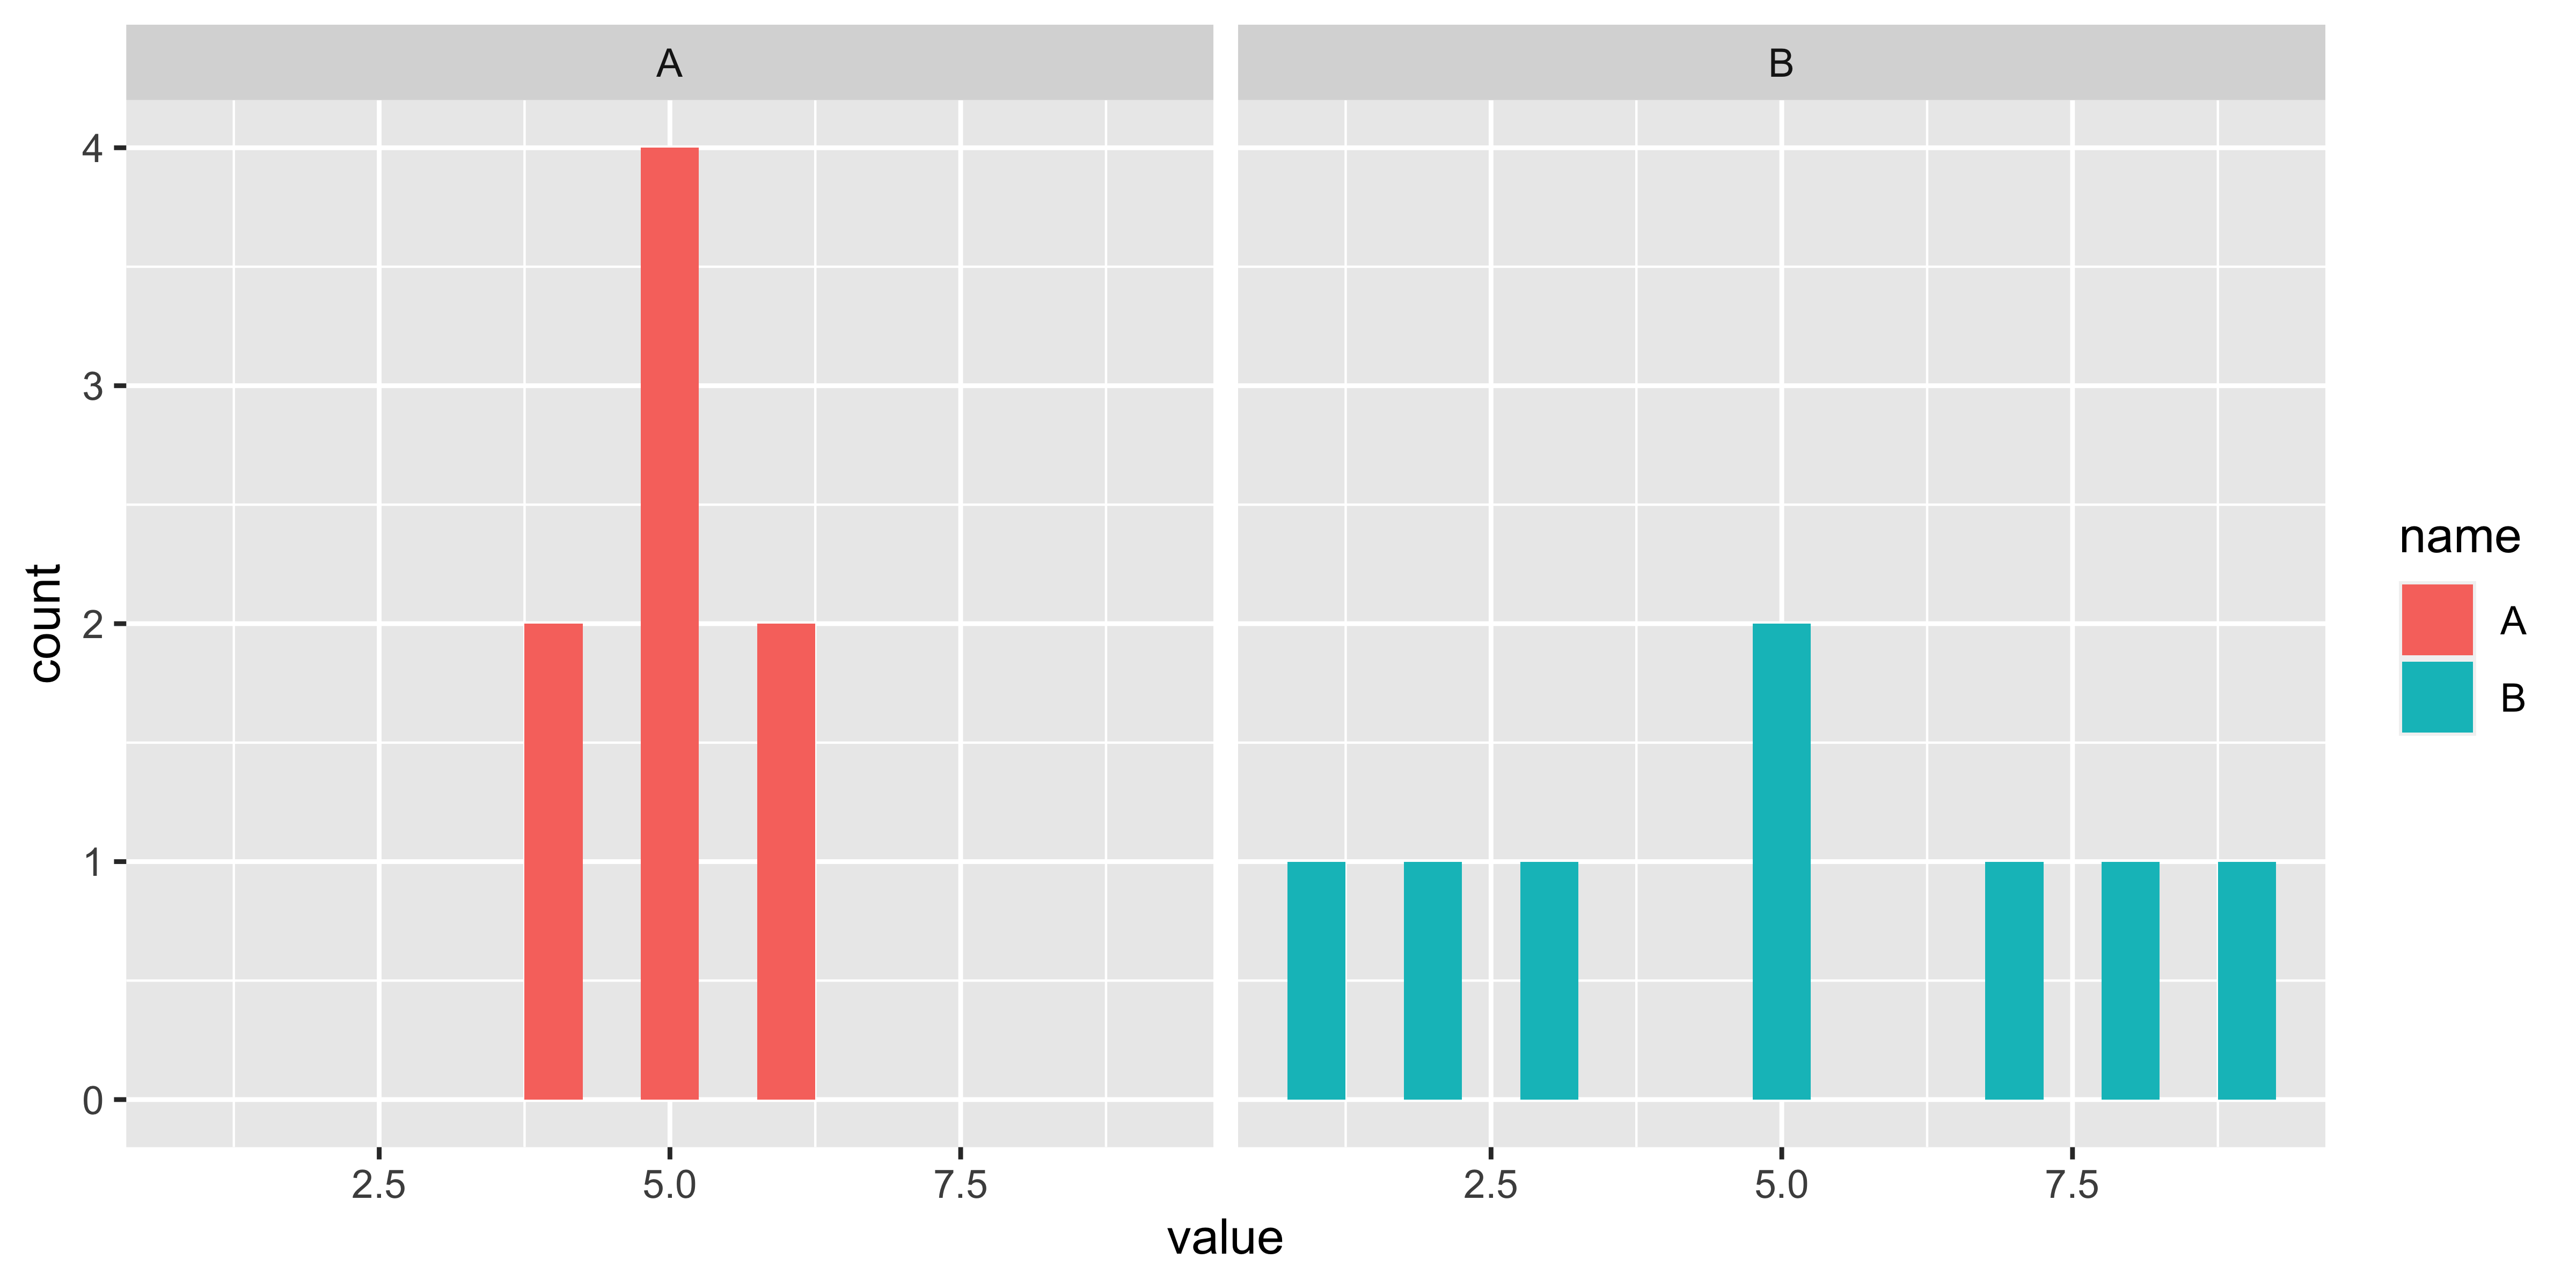
\includegraphics[keepaspectratio,width=12cm]{images/text04/Rplot04_01.png}
        \caption{二つのデータを見比べてみよう}
        \label{fig::04_04}
    \end{figure}

このデータ，A/Bグループについてそれぞれ平均値，中央値，最頻値はどうなるでしょう。何と，平均値はA群もB群も5，中央値もA/B群ともに5，最頻値もA/B群ともに5となります。中心化傾向の指標だけでは，A群とB群の違いが表現できません。こんなにも違う見た目をしているのに！

この2つの群は何が違うかといって，図\ref{fig::04_05}を見れば明らかなように中心から左右にどれほど散らばっているかが違うのです。

\begin{figure}[ht]
    \centering
    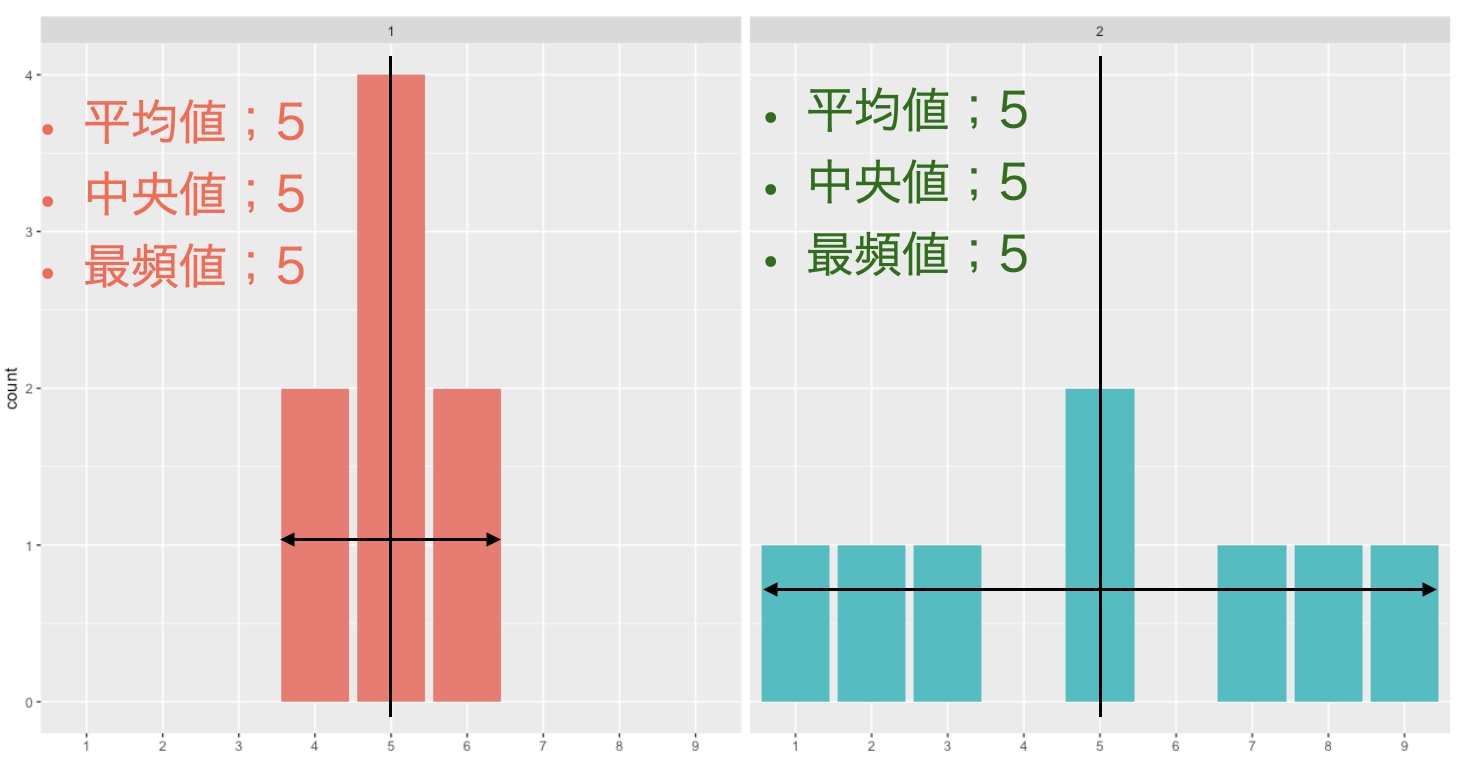
\includegraphics[keepaspectratio,width=12cm]{images/text04/slide04_05.png}
    \caption{中心から各データ点が平均的にどの程度離れているか}
    \label{fig::04_05}
\end{figure}

\paragraph{分散}
これをうまく表現する代表値は，\textbf{分散variance}があります。指標化のポイントは，「中心から個々のデータ点が平均的にどの程度離れているか」を考慮することにあります。数式では次のように表されます。

$$ s_x^2  = \frac{1}{N}\sum_{i=1}^N (x_i - \bar{x})^2 $$

この式にある$(x_i - \bar{x})$は，各データ点$x_i$が平均$\bar{x}$から離れている程度を表しています。これを特に\textbf{平均偏差}と言います。それを二乗していますね。これがポイントで，二乗しておかないと平均偏差の総和はゼロになってしまうからです\footnote{検算してみよう!}。プラスとマイナスが打ち消し合うからゼロになってしまうわけで，符号の影響をなくすべく二乗しているのだと思ってください。符号をなくすのには絶対値でもいいのですが，絶対値は数式で書けないから使いにくいのです\footnote{絶対値は$|x|$と書くじゃないか，と思った人もいるかもしれません。おしい，もう一歩。この記号の中身，計算式を考えてみてください。$0\le x$のとき，$|x|=x$です。$x<0$のとき，$|x|=-x$です。これ，「・・・の時」という条件で分岐してて，この箇所が数式で書けてないですよね。}

実際に計算してみましょうか。A群の分散は，次のようになります。
$$\frac{1}{8}((4-5)^2+(4-5)^2+(5-5)^2+(5-5)^2+(5-5)^2+(5-5)^2+(6-5)^2+(6-5)^2)$$
$$=\frac{1}{8}(1^2+1^2+0^2+0^2+0^2+0^2+1^2+1^2) = \frac{4}{8}=0.5$$
B群の分散は，次のようになります。
$$\frac{1}{8}((1-5)^2+(2-5)^2+(3-5)^2+(5-5)^2+(5-5)^2+(7-5)^2+(8-5)^2+(9-5)^2)$$
$$=\frac{1}{8}(4^2+3^2+2^2+0^2+0^2+2^2+3^2+4^2) = \frac{58}{8}=7.25$$
このように，A群の分散は0.5，B群の分散は7.25と，B群の方が散らばりが大きいことがわかります。

分散はデータの散らばりを表現しています。分散が大きい方がデータの散らばりが大きい，というわけですね。
逆に分散がゼロになると，そのデータには散らばりがない，ということです。
実際撮ったデータの分散がゼロだと，そこから得られる情報がない，ということになります。
なぜなら，例えばクラスの全員がテストで100点を取ると，分散は0です。この時は「どういう勉強をすれば成績が上がるか」とか「成績が低い人をどうサポートすれば良いか」という知見を得ることができません。分散が0のデータセットには，個々の違いがないので情報が得られないのです。つまり，分散はそのデータから取り出せる「意味」「情報」の上限という点で非常に重要な指標なのです！

\paragraph{標準偏差}
ところで，分散は元のデータを二乗した値から計算しているのでした。ですから，その単位が元の尺度と異なることに注意が必要です。つまり，元がcm位のデータであれば，分散は$cm^2$の単位になっているのです。ですから数字が必然的に大きくなりがちですし，分散の大きさが実際どれぐらいなのか，という実感が持ちにくいという欠点があります。

そこで，単位を元に戻すことを考えます。二乗して大きくなっているのですから，平方根を撮ってやれば元に戻りますね。
$$ s_x = \sqrt{\frac{1}{N}\sum_{i=1}^N (x_i - \bar{x})^2} $$
このようにして計算された$s_x$のことを\textbf{標準偏差standard deviation,SD}と言います。これはルートを取るだけですので，すぐに計算できますね。先程の例ですと，A群のSDは0.7071，B群のSDは2.6925です。

\section{データの相対的位置}
平均値と標準偏差を導入したことで，データ点の相対的位置を表現することが可能になった。心理学の研究対象の多くは，絶対ゼロ点をもたない間隔尺度水準であり，個々のデータ点の特徴を記述する際には相対的な位置である標準得点で表されることが多い。ここでは標準化の方法と標準得点の特徴，標準得点の応用である偏差値の特徴および算出方法について理解する。
\begin{flushright}
    $\to$ \citet{山内201001}のP.54--56,\citet{Yamada2004}のP.38--41，\citet{川端201408}のP.36--40。
\end{flushright}

\section{変数間関係の指標}ここまでは1つの変数についての特徴を記述するものであったが，次に複数の変数による変数同士の関係を考える。1つは共分散であり，それを標準化したスコアにしたものが相関係数であることを理解する。また相関係数はあくまでも変数間の直線的関係についての記述であり，相関係数だけを見て判断すると対象の理解を誤る場合があることに注意する。
\begin{flushright}
    $\to$ \citet{山内201001}のP.62--75,\citet{Yamada2004}のP.44--59，\citet{川端201408}のP.48--58。
\end{flushright}

\section{課題}
\paragraph{変数を見つける}次のような研究計画を立てた時に，変数として記録しておくべきなのは何でしょうか。
\paragraph{尺度水準を理解する}次のそれぞれのデータは，どの尺度水準に該当するでしょうか。
\begin{enumerate}
\end{document} 
